\documentclass[runningheads]{llncs}
\usepackage[T1]{fontenc}
\usepackage{graphicx, amsmath, amssymb, stmaryrd, seqsplit, float}
\usepackage{placeins}
\usepackage{tikz}
\graphicspath{{../../graphs/}{graphs/}{./}}
\let\proof\relax
\let\endproof\relax
\usepackage{amsthm}

\begin{document}
%
\title{Vn-IPFS: Re-engineering IPFS using von Neumann's Reliable Organism Synthesis Principles}
%
%\titlerunning{Abbreviated paper title}
% If the paper title is too long for the running head, you can set
% an abbreviated paper title here
%
\author{Justin Y. Shi \inst{1}
\email{shi@temple.edu}
\orcidID{0000-0003-3774-2190}
\and
Nick Tagliamonte \inst{1}
\email{tug35742@temple.edu}
\orcidID{0009-0008-3300-1057}
\and
Garrett Stoll \inst{1}
\email{tuv14706@temple.edu}
\orcidID{0009-0007-6819-1156}
}
%
\authorrunning{J. shi \& N. Tagliamonte \& G. Stoll}
% First names are abbreviated in the running head.
% If there are more than two authors, 'et al.' is used.
%
\institute{Temple University, Philadelphia PA 19102, USA}

\maketitle              % typeset the header of the contribution
%
\begin{abstract}
    This paper presents vn-IPFS, a decentralized file system featuring N-hop asynchronous replication and complete peer-to-peer protocols with modified DHT or centralized coordinator. Evaluation on multi-daemon testbeds demonstrates deterministic peer formation and stable replication across increasing node counts, with logarithmic scaling of propagation depth ($O(\log_k N)$) and low variability. The design achieves robust replication by utilizing UVR-synchronized tuple-space coordination as a substrate for topology-constrained replication. The system enforces a minimum of seven replicas per file and verifies retrieval via majority content-hash consensus, yielding Byzantine fault tolerance ($3f+1$) for content integrity within each connected component. Each coordination tuple implicitly triggers a self-check at the receiver to maintain \(N\ge 7\) with customizable replication targets and without explicit failure detection.
    \keywords{Peer-to-Peer Systems \and Decentralized Replication \and N-Hop Replication \and Gossip Protocols \and Distributed Tuple Space \and libp2p \and Overlay Networks}
\end{abstract}
%
%
%
\section{Introduction}
In content-addressable peer-to-peer systems, simply ``publishing'' a file does not guarantee that it meaningfully diffuses through the network. Popular approaches rely on global routing tables (e.g., DHTs \cite{StoicaChord01}) that encourage replication to remain clustered near the originator. While DHTs nominally offer random distribution, production optimizations like Proximity Neighbor Selection (PNS) cause logical neighborhoods to correlate with physical geographic regions, introducing regional concentration vulnerabilities. Systems like Ethereum Swarm employ Kademlia-based DHTs with nearest-neighbor replication, where replicas cluster in topological neighborhoods, creating regional concentration vulnerabilities (see Section~\ref{sec:related-work} for detailed comparison). These approaches also struggle under churn and network partitions, where global state is incomplete and connectivity is transient. The result is an ecosystem in which replication can be opportunistic but not principled: it is difficult to enforce where replicas live, and harder still to guarantee that replicas are separated by meaningful topological distance.
This paper presents vn-IPFS, which uses DHT with a revised hashing scheme for Tuple Space implementation in order to decouple providers from data contents. The data contents are directly hashed as keys for search. These keys enable concurrency control, replication control and automatic de-duplication. By enforcing N-hop exclusion, we drive replicas outward from the uploader's neighborhood to improve fault isolation. This architecture strictly separates coordination (tuples) from transport (bytes), ensuring that control-plane stability is maintained even when data bandwidth is saturated, preventing "route flapping" common in coupled P2P systems. Our evaluation confirms that propagation depth scales logarithmically ($O(\log_k N)$) with network size.
The DHT layer implements von Neumann principles of reliable system construction in a distributed setting: keys are stateless with respect to the global topology (each tracks only its peers), and failed provider nodes are bypassed automatically. Global routing invariants are maintained without the fragility under churn, vnIPFS relies on statistical convergence through parallel message paths: multiple physical paths operate concurrently, and coordination emerges from the aggregate behavior of these paths rather than from strict structural guarantees. File persistence and replication liveness under churn—even in the presence of malice—are ensured at the content layer: per-message self-checks with majority content-hash excise nodes that lose or altered files by re-replicating their manifests to sustain at least seven replicas. On top of this substrate, replication intent and status propagate as tuples; nodes that satisfy the N-hop customizable constraint fetch the file directly over libp2p and publish completion tuples. This file system architecture avoids global routing tables and single points of control while providing a principled, topology-aware replication policy that operates across partitions.
We build an end-to-end system and a reproducible test harness. Our evaluation demonstrates deterministic ring formation and stable replication across increasing node counts, with logarithmic scaling of propagation depth ($O(\log_k N)$) and low variability. These results show that UVR-synchronized tuple-space coordination is a practical substrate for topology-constrained replication in dynamic, partitioned networks. This aligns with established eventual-consistency practice \cite{Burckhardt2014EC}.
This paper makes the following contributions:
\begin{itemize}
    \item Complete provider decoupling from data contents via direct content hash keys.
    \item Direct content keys are used for concurrency control to prevent race conditions, replication controls and automatic data de-duplication.
    \item A topology-aware replication policy with N-hop exclusion that balances access performance, security and diffusion beyond the originator’s neighborhood.
    \item A DHT-coordinated tuple-space substrate that provides stateless content maintenance, automatic failure bypass/repair, and convergence under churn, aligning with von Neumann reliability principles.
    \item A complete separation of concerns between coordination (tuples via DHT) and transport (libp2p), yielding a clean, testable implementation boundary.
    \item Content-integrity consensus via a majority content-hash across replicas with a system-wide minimum of seven copies per file, providing Byzantine fault tolerance for content integrity.
    \item An end-to-end implementation and benchmark harness demonstrating stable operation and logarithmic propagation-depth scaling ($O(\log_k N)$) across multi-daemon tests.
\end{itemize}

\section{Related Work}
\label{sec:related-work}
Distributed content routing and placement has been dominated by DHT-based overlays (e.g., Chord/Kademlia families \cite{StoicaChord01}), which optimize lookup via structured, global routing tables but couple distant nodes and require continual repair under churn. Gossip-style dissemination provides scalable aggregation and fault tolerance without global invariants \cite{Jelasity2005Gossip}, while CRDT-style, lattice-based state convergence offers idempotent, monotone merges and eventual consistency guarantees \cite{ShapiroCRDT2011,BaqueroPureOpCRDT2017,Burckhardt2014EC}. Monitoring overlays such as Astrolabe summarize global state with compact per-node views \cite{Astrolabe2003}. Our approach combines a minimal neighbor-only ring overlay (UVR) to bias gossip with a tuple-space coordination plane that adopts CRDT principles for monotone, convergent state; unlike DHTs, we target placement and diffusion (N-hop exclusion), not sublinear lookups, and avoid global routing tables and their repair obligations.

\subsection{Kademlia and Swarm: DHT-Based Content Storage}
Kademlia \cite{StoicaChord01} provides a distributed hash table that maps keys to values using XOR-distance routing in a structured overlay. Systems like Ethereum Swarm leverage Kademlia for content-addressable storage, where content identifiers (CIDs) are mapped to node addresses in a shared 256-bit address space. The \emph{proximity principle} governs placement: nodes store chunks whose addresses are numerically closest to their own overlay address, creating neighborhoods of nodes responsible for overlapping address ranges.

\paragraph{Routing State Architecture.}
It is important to distinguish between routing state and content replication. In standard DHTs like Kademlia and Chord, routing tables are \emph{partitioned}, not replicated: each node maintains a unique partial view of the network (e.g., k-buckets in Kademlia, finger tables in Chord), containing dense local information and sparse global information. The global routing capability emerges from the aggregation of these partial views, not from replication of a master table. Specialized architectures like OneHop DHTs employ full table replication (every node knows every other node) to achieve $O(1)$ lookups, but at prohibitive bandwidth cost for large networks. vn-IPFS leverages DHT routing tables for direct content searches. Once the data target is found, data transfers are implemented via direct swarms.

\paragraph{Nearest-Neighbor Replication.}
Swarm and similar Kademlia-based systems employ nearest-$k$-neighbor replication, where $k$ nodes in the same neighborhood maintain copies of each chunk. This approach provides redundancy within a topological region but does not enforce geographic or network-topological separation. Replicas cluster near the content's hash address, creating regional concentration: if all $k$ replicas reside in a single geographic region or network partition, regional outages (natural disasters, network partitions, or coordinated attacks) can render content inaccessible despite nominal redundancy. vnIPFS leverages the overlapping routing tables for fault tolerance under churn. Lookups can only fail when all replicated entries disappear at the same time.

\paragraph{Coordination and Transport Coupling.}
In Kademlia-based systems, coordination (routing decisions) and transport (data transfer) are tightly coupled: retrieval requires traversing the DHT to locate providers, and placement follows the proximity principle deterministically. This coupling creates dependencies: routing table repair must complete before reliable placement or retrieval can proceed. Systems like Swarm address this with protocols like Push-Sync (forwarding chunks toward their target neighborhood) and Pull-Sync (gossip-based replication within neighborhoods), but these still rely on the underlying DHT structure for initial routing decisions. Additionally, DHT-based systems often require Merkle tree validation for content integrity, which adds logarithmic complexity ($O(\log_2 N)$) to retrieval operations and can significantly impact response time, particularly as the content structure grows.

\paragraph{Comparison with vn-IPFS.}
Our design makes different architectural choices that address the limitations while preserving the benefits of decentralized, content-addressable storage. \emph{Placement policy:} Search keys are direct hash of contents. All accesses to the content to the matching key can be serialized via the key. The key also serves as replication controller. Instead of nearest-neighbor clustering, vn-IPFS enforces a customizable N-hop exclusion that can balance performance, security and extreme fault tolerance by explicitly pushing some replicas away from the originator's immediate neighborhood. This diversity-aware replication promises to deliver high performance content retrieval and extreme fault isolation: replicas are separated by meaningful topological distance, reducing the probability that a single regional event affects all copies. A typical N-hop exclusion policy is 40-30-30 with 40\% replicas in the nearest neighbors, 30\% in medium range and 30\% in far-flong networks. \emph{Coordination substrate:} We use DHT to implement tuple-space coordination layer. This automates global routing table updates; coordination state converges via gossip while maintaining routing invariants. \emph{Separation of concerns:} Coordination (replication intent, status) flows as tuples; data transfer occurs directly over libp2p when a key is locked and nodes accept replication request. This separation localizes failures: routing table degradation does not block data transfer, and transport failures do not corrupt coordination state.

Table~\ref{tab:swarm-vnipfs} summarizes the placement and locality contrasts between Ethereum Swarm's DISC (distributed immutable storage of chunks) and vn-IPFS along the dimensions that most affect durability under regional failures.

\begin{table}[t]
\caption{Placement and locality: Ethereum Swarm (DISC) vs.\ vn-IPFS.}
\label{tab:swarm-vnipfs}
\centering
\begin{tabular}{@{}lp{4.1cm}p{4.1cm}@{}}
\hline
\textbf{Feature} & \textbf{Ethereum Swarm (DISC)} & \textbf{vn-IPFS} \\
\hline
Placement Logic & Neighborhoods: nodes store chunks whose XOR address is close to their own address. & N-Hop Exclusion: nodes store files if they are $N$ hops away from the source in the overlay. \\
Locality & Optimizes for retrieval latency. Replicas cluster logically (and via PNS, physically). & Optimizes for fault isolation. Replicas are forced apart topologically. \\
Diversity Guarantee & Probabilistic (depends on ID distribution). & Structural (enforced by hop counting). \\
Vulnerability & Susceptible to regional outages if PNS is aggressive. & Higher latency for retrieval, but robust against regional partitioning. \\
\hline
\end{tabular}
\end{table}

\paragraph{Trade-offs and Complementary Strengths.}
Kademlia-based systems excel at sublinear lookup performance ($O(\log N)$) and benefit from decades of optimization and deployment experience. vn-IPFS trades lookup speed for replica diversity and fault isolation: we prioritize ensuring replicas are topologically separated over minimizing retrieval latency. The tuple-space coordination model introduces additional control traffic compared to direct point-to-point coordination, but simplifies failure handling and eliminates global table repair. Both approaches can coexist: Kademlia remains superior for applications requiring fast, structured lookups with regional clustering acceptable; vn-IPFS targets scenarios where replica diversity and partition resilience are paramount, and where the coordination overhead is acceptable for the improved fault isolation guarantees.

\section{Motivation and Comparison to DHT-based Designs}
Mainstream content-addressable systems (e.g., IPFS, Ethereum Swarm) rely on DHT-style content routing (Chord/Kademlia families \cite{StoicaChord01}). Section~\ref{sec:related-work} provides a detailed technical comparison with Kademlia-based systems, particularly Swarm, examining nearest-neighbor replication, coordination-transport coupling, and regional constraint vulnerabilities. Our design makes a different choice on first principles, prioritizing replica diversity and fault isolation over sublinear lookup performance.

\paragraph{Why DHT is Not Good.}
\emph{Global routing tables.} DHTs maintain structured, global routing tables to guarantee $O(\log N)$ lookups via <provider, data> hashes. A replicated data item will have multiple hashes. When the provider crashes or corrupts data, or new providers become available, the global routing tables must be repaired. Maintaining those invariants under churn, partitions, and asymmetric connectivity imposes global dependencies and continual table repair. \emph{Von Neumann guidance.} We favor local composition with minimal cross-coupling: the DHT-Tuple Space uses only data content keys and provider pointers and gossip-synchronized swarm transfers. DHT-wide invariants couple distant nodes;  neighbor-only invariants preserve locality and statelessness. \emph{Operational centralities.} Real deployments concentrate control at well-known bootstrap endpoints and shared pinning/gateway services; these become de facto single points of failure or control, even if the data plane is nominally decentralized.

\paragraph{Practical implications.}
\emph{Placement vs. lookup.} DHTs optimize lookup latency, not placement. Kademlia-based systems like Swarm employ nearest-$k$-neighbor replication, where replicas cluster in topological neighborhoods near the content's hash address; this creates regional concentration where all replicas may reside in a single geographic region or network partition (see Section~\ref{sec:related-work}). Our N-hop policy explicitly pushes replicas outward, improving fault isolation and load dispersion. \emph{Behavior under partitions.} DHT maintenance assumes eventual global re-stitching; lookups may return stale or empty under split-brain. DHT with tuple space operates per-data: progress and safety are stated per tuple (key), then reconcile on re-merge. \emph{Failure surfaces.} DHT routing tables degrade with churn; eclipse and hotspot risks are well known. DHT-Tuple Space confines data state to neighbor pointers; failures trigger bounded local repair.

\paragraph{Summary.}
Our goal is reliable, topology-aware replication with strict separation of content coordination (tuples (keys)) and data transport (libp2p). DHT routing provides an efficient global routing layer. With Tuple Space semantics, the routing table repairs are also automated; we enforce N-hop exclusion at the data replication layer. This aligns with von Neumann-style construction: small, local invariants with monotone, convergent coordination.

\section{DHT Tuple-Space Coordination Semantics}
Replication intent and state live in a Synergy tuple space and are synchronized over a modified DHT search engine. Each node maintains a local routing table with $k$ peers (e.g., $k\approx 20$); in $h$ hops the system can reach on the order of $k^h$ nodes—e.g., $20^5 \approx 3.2\times 10^6$, scaling practically to internet-wide participation. Each message from a source can be traced back to the originator along its path, yielding a globally stable total order of messages (and thus of transactions) without central coordination. Each node maintains only local peers and stores received ``upload/replicate" message origins and local state. Each node may terminate a message by responding to the request and complete its acknowledgment, or forward the message along its peers, creating multiple parallel paths that collectively enable coordination without global routing tables. DHT-Tuple Space provides a small set of primitives—peer maintenance and best‑effort tuple spread—on which vn‑IPFS builds init, table management, and replication. The coordination layer follows a lattice‑based eventual consistency model with idempotent merges and keeps transport separate. This matches CRDT practice for monotone, convergent state \cite{ShapiroCRDT2011,BaqueroPureOpCRDT2017}, uses gossip‑style dissemination suitable for large, dynamic networks \cite{Jelasity2005Gossip}, and aligns with established eventual consistency principles \cite{Burckhardt2014EC}. Compact ring‑info summaries also fit the spirit of monitoring overlays like Astrolabe \cite{Astrolabe2003}. The approach is orthogonal to mixed‑consistency systems (e.g., MixT \cite{MilanoMyersMixT2018}).

\subsection{Architecture and Interfaces}
Initialization binds identity to DHT participation. The init request (UID, AppID, host/port, PID) mirrors the Synergy C layout (\texttt{uvr\_init\_it}); the response reports counts, next-hop metadata, and status. Per-node facts live in \texttt{HostInfo} (IP, AppID, UID, PID, resources, status) for topology and publication. Before coordinating, \texttt{UVRManager} confirms reachability to TSH via a TCP handshake. It then emits init/ping tuples (\texttt{\seqsplit{uvr\_init\_<AppID>\_<PID>}}, \texttt{uvr\_ping\_<AppID>\_<PID>}) and polls \texttt{uvr\_ring\_info\_<AppID>} with bounded timeouts so all state reflects the live, gossip-synchronized ring.

\subsection{Ring Formation, Maintenance, and State Publication}
The ring manager maintains order and predecessor/successor maps; supports init/join/leave; and updates version, status, and timestamps. It offers traversal (\texttt{\seqsplit{TraverseRing}}), O(1) next/prev, and targeted repair; duplicate joins by the same AppID are rejected. The integration layer runs discovery and repair workers and exposes topology and statistics. On each update it publishes \texttt{uvr\_ring\_info\_<AppID>} with \{total\_nodes, ring\_version, timestamp\}, giving an externally visible, eventually consistent ring size for init/ping and tests. Liveness/consistency does not use heartbeats or traversal workers: upon receipt of any coordination tuple, a node self-checks its manifest and repairs missing/divergent content via majority content-hash, maintaining \(N\ge 7\) without explicit failure detection. Rather than enforcing strict structural invariants that create fragility under churn, the system relies on statistical convergence: multiple parallel UVR message paths operate concurrently, and coordination state emerges from the aggregate behavior of these paths. Local neighbor relationships plus global summaries let the system converge under churn while remaining inspectable.

\subsection{Replication and Transport Separation}
Replication intent moves hop-by-hop as tuples addressed to targets. For remote placements, the manager emits \texttt{\seqsplit{replicate\_request:<node\_id>:<request\_id>}} with a compact payload (CID, hop counters, creator, timestamp). Tuple-space writes are best-effort: if a write fails or a message is dropped, the sender retransmits until the tuple is accepted or a bounded TTL is exhausted; this matches the channel model (Communication/Fairness) assumed in the convergence and liveness proofs below. A background receiver on each node polls for local requests and triggers idempotent processing. On acceptance, the node fetches the file from the originator (or a predecessor) via libp2p when available (\texttt{\seqsplit{RequestFile(originator, CID)}}), with a minimal shared-file fallback if needed. Completion updates local state and may be echoed in tuples. Coordination (intent/progress/summaries) stays in the tuple space; bytes flow over libp2p, keeping the layers separate and failure-isolated. This separation contrasts with Kademlia-based systems where coordination and transport are tightly coupled: retrieval requires traversing the DHT to locate providers, creating dependencies where routing table repair must complete before reliable placement or retrieval can proceed (see Section~\ref{sec:related-work}). The system enforces a minimum of seven replicas for every file and verifies retrieval via majority content-hash among available replicas before returning bytes. Upon receipt of any coordination tuple, the receiver performs a self-check of its manifest and, if necessary, repairs missing or divergent content according to the majority hash, thereby maintaining \(N\ge 7\) with global balance but without ring traversal or explicit failure detection. If a node's local content disagrees with the majority for any \(\mathit{cid}\), it re-emits replication requests for its manifest to preserve \(N\ge 7\) global balance and then shuts down, removing potentially faulty or malicious sources without central revocation while maintaining durability.

\section{Replication Theory: N-Hop Exclusion and Content Consensus}
We model the network as a graph \(G=(V,E)\), where vertices are peers and edges are live links. The UVR layer induces a logical ring \(R=(V,A)\) with predecessor/successor pointers only. Replication tasks are through message tuples \\
$T=(\mathit{cid}, n, \mathit{excluded}, \mathit{originator})$,
\\
propagated by the tuple space synchronized over multiple parallel UVRs.

\subsection{Policy and Mechanism}
The goal is to place \(n\) replicas on nodes that are both nearby and lie outside the originator's immediate neighborhood—enforcing topological separation without centralized knowledge. The system enforces a global minimum \(n\ge 7\) in all scenarios. This threshold follows Byzantine fault tolerance theory: tolerating \(f\) Byzantine faults requires \(3f+1\) replicas; with \(n=7\), the system can tolerate \(f=2\) malicious nodes while maintaining a strict majority of honest replicas for consensus. The uploader initializes a tuple with remaining replica count and a customized exclusion set seeded with itself (and locally known neighbors). As tuples propagate, each node evaluates eligibility locally. A node \(r\) may accept if it is not excluded, has not stored \(\mathit{cid}\), and \(n>0\). The originating node is responsible for the final decision. On acceptance, \(r\) fetches the file directly from the originator, stores it, responds with a completion acknowledgment. A timeout on the acknowledgment will disqualify the replica in favor for the next candidate. The originator then manages all candidates according to the N-hop exclusion policy. The process halts when \(n=0\) the entire replication vector is satisfied. This local, monotone exclusion drives replicas to nearby nodes and away from the uploader and discourages clumping. Unlike nearest-neighbor only replication in Kademlia-based systems (where replicas cluster in topological neighborhoods), N-hop exclusion ensures replicas are separated by meaningful graph distance, satisfying high performance retrieval while reducing the probability that regional outages or network partitions affect all copies simultaneously.

\subsection{Diffusion, Substrate, and Guarantees}
Exclusion updates approximate an \emph{N-hop frontier}: by  disqualifying peers for new replicas, forcing a globally balanced performance (through the shortest distance knowledge) and reliability measure through subsequent acceptances occur at increasing graph distance in expectation. UVR supplies the convergent substrate: stateless neighbor maintenance under churn and deterministic ring order for message tuple propagation \cite{Jelasity2005Gossip}. Under eventual tuple propagation in a connected component \cite{Burckhardt2014EC}, liveness follows—eligible nodes eventually observe applicable tuples; bounded TTL/retry prevent indefinite stalls. Safety follows from local idempotence and non-decreasing exclusion sets \cite{ShapiroCRDT2011}; the target is met when the remaining count reaches zero. In partitions, replication proceeds independently within components; when connectivity returns, UVR re-converges and tuple TTL/versioning prevents unbounded replay. For content integrity, retrieval performs a \emph{majority content-hash} across available replicas; the majority digest is returned and any divergent local copy is discarded. This enforces immutability semantics (a modified byte sequence is a new object with a new CID) and yields Byzantine fault tolerance for content integrity provided a strict majority of the seven-or-more replicas are honest. Unlike systems like Swarm that rely solely on cryptographic validation (verifying content against a Merkle root hash), vn-IPFS adds a democratic consensus layer: validity is determined by network agreement, not just cryptographic verification. This is particularly relevant for detecting widespread corruption or coordinated attacks that might bypass simple hash checks. The N-hop exclusion policy provides additional defense against excessive faults: an attacker attempting to control a majority of replicas (4 out of 7) cannot simply cluster malicious nodes locally; they must control nodes distributed widely across the entire network, significantly increasing the attack's coordination difficulty.

\subsection{Complexity and Practicality}
Per-node UVR state remains \(O(1)\). Propagation complexity is \(O(\log_k N)\) in hop count, where \(k\) is the average peer count per node, rather than \(O(N)\): reach at \(h\) hops is on the order of \(k^h\) nodes, so to cover a network of size \(N\) we need \(h\) such that \(k^h \geq N\), i.e., \(h = O(\log_k N)\). This \(({\mathit{peercount}})^{({\mathit{hopcount}})}\) metric provides the theoretical bound for dissemination depth. Coordination cost grows with accepted replicas and bounded observation rates; measured propagation depth exhibits logarithmic scaling ($O(\log_k N)$) in practice. Transport cost is dominated by file size and count of successful transfers; separation of concerns keeps coordination progress robust to transport variance and failures.

\section{Formal Proofs}
We keep two core formal results fully stated (finite-height convergence on a quiescent epoch; replication liveness within a connected component) and condense peripheral arguments as proof sketches.

\subsection{Notation and Illustrative Examples}
To make the notation concrete, consider a simple undirected graph with six nodes and ring-like connectivity. Distances $d(u,v)$ are hop counts, $B(v,r)$ is the set of nodes within $r$ hops, and $S(v,r)$ is the ring of nodes at exactly $r$ hops. The exclusion frontier $E_k$ grows by taking unions of closed balls $B(a_i,h)$ around accepted nodes $a_i$.

\begin{figure}
  \centering
  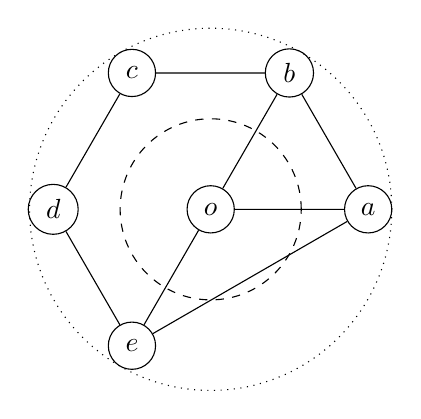
\begin{tikzpicture}[scale=1, every node/.style={circle, draw, minimum size=6mm}]
    \node (o) at (0,0) {$o$};
    \node (a) at (2,0) {$a$};
    \node (b) at (1,1.732) {$b$};
    \node (c) at (-1,1.732) {$c$};
    \node (d) at (-2,0) {$d$};
    \node (e) at (-1,-1.732) {$e$};
    \draw (o)--(a)--(b)--(c)--(d)--(e)--(o)--(b);
    \draw (a)--(e);
    % illustrative shells
    \draw[dashed] (0,0) circle [radius=1.15];
    \draw[dotted] (0,0) circle [radius=2.3];
  \end{tikzpicture}
  \caption{Toy topology for notation: $d(\cdot,\cdot)$ counts hops; dashed/dotted circles illustrate shells around $o$.}
\end{figure}
\FloatBarrier

\subsection{Model and Assumptions}
\paragraph{Processes and Graph.} We consider a finite set of nodes $V$ and a time-varying directed graph $G_t=(V,E_t)$ describing who can talk to whom. After a quiescent time $T$ (defined below), each connected component is strongly connected and its membership stops changing.
\paragraph{Asynchrony.} The system is asynchronous: message and processing delays are finite but unbounded; there are no global clocks or rounds.
\paragraph{Failure Model.} Coordination proofs assume crash/omission faults (non‑Byzantine): a crash halts a node; omissions drop messages. For content integrity, retrieval applies a majority content‑hash across replicas: with at least seven replicas per $\mathit{cid}$ and a strict honest majority among the available replicas, the majority digest is returned, any divergent local copy is repaired, and the violator self‑quarantines by re‑emitting replication intents for its manifest and shutting down. We reason about nodes that are alive after time $T$.
\paragraph{Content‑Integrity Assumption.} Files are immutable and content‑addressed (a modified byte sequence yields a new $\mathit{cid}$). On retrieval within a connected component, among the available replicas of a $\mathit{cid}$, a strict majority are honest. Majority content‑hash selection therefore yields Byzantine fault tolerance for content integrity and does not alter the coordination assumptions (A1–A6) used below.
\paragraph{Communication.} Channels are best-effort: senders may retransmit. Payloads are elements $m\in L$ (see below). If retransmissions are bounded (TTL), our guarantees apply to payloads retransmitted indefinitely under fairness.
\paragraph{Fairness.} After $T$, within any component $C$, any payload content that is retransmitted infinitely often is delivered to every node in $C$ infinitely often. This rules out perpetual starvation while allowing finite losses and reordering.
\paragraph{State and Merge.} Each node $v$ holds state $x_v$ in a finite join-semilattice $(L,\sqsubseteq,\sqcup)$. On receipt of $m\in L$, it updates $x_v\gets x_v\sqcup m$. The join is associative, commutative, idempotent, and monotone.
\paragraph{Fact Injections.} Applications may add new facts before $T$. After $T$ (the quiescent epoch), no new facts are injected. We analyze convergence for $t\ge T$.
\paragraph{API Semantics.} \textsc{Put} inserts a fact (before $T$). \textsc{Get} returns the current state $x_v$. Both are at-most-once at the application level; network duplication is absorbed by idempotence.
\paragraph{UVR Ring Abstraction.} UVR is not a single literal ring but a parallel message-passing abstraction: every message path through peers forms a UVR, and these paths operate concurrently. The abstraction $R=(V,A)$ biases gossip through neighbor links, where $A$ represents predecessor/successor relationships that enable multiple parallel message paths.
\emph{UVR properties:} (i) every live node maintains exactly one predecessor and one successor pointer; (ii) no self-loops; (iii) messages propagate along neighbor links, creating multiple parallel UVR paths per component; (iv) failed nodes are bypassed through neighbor repair, allowing new paths to form. Rather than enforcing strict structural invariants, UVR relies on statistical convergence: coordination emerges from the aggregate behavior of parallel message paths rather than from global structural guarantees.

\paragraph{Assumptions (A1–A6).}
$\newline$ A1: After time $T$, within a component $C$ the communication graph is strongly connected.
$\newline$ A2: Fair delivery: any payload retransmitted infinitely often is delivered to every node in $C$ infinitely often.
$\newline$ A3: Best-effort retransmission without effective TTL for the target tuple.
$\newline$ A4: Greedy, idempotent acceptance: an eligible node accepts once upon observing $n>0$.
$\newline$ A5: Exclusion monotonicity: acceptance adds the node to $\mathit{excluded}$ permanently.
A6: Capacity: at least $n$ distinct live nodes in $C$ are eligible at time $T$ and remain live.

\subsection{Tuple-Space Convergence on a Quiescent Epoch}
\begin{theorem}[Finite-Height Convergence on a Quiescent Epoch]\label{thm:finiteheight}
Let $(L,\sqsubseteq,\sqcup)$ be a finite join-semilattice and let each node
$v$ hold a state $x_v(t)\in L$ at time $t$.
Suppose updates are of the form $x_v \gets x_v \sqcup m$ upon message delivery.
Fix a time $T$ after which (i) no new facts are injected, and
(ii) within each connected component $C$ of the communication graph,
the component is strongly connected and message delivery is fair
(any payload retransmitted indefinitely is delivered to every node in $C$ infinitely often).
Define
\[
J \;=\; \bigsqcup_{u\in C} x_u(T).
\]
Then there exists $T'\ge T$ such that for all $t\ge T'$ and all $v\in C$ we have
$x_v(t)=J$. In particular, each sequence $(x_v(t))_{t\ge T}$ is monotone, admits at most
$\lvert J\rvert$ strict increases, and stabilizes in finite time.
\end{theorem}

\begin{proof}
\textbf{(1) Monotonicity and bound.} Every update is $x\to x\sqcup m$, hence $x\sqsubseteq x\sqcup m$. After $T$ no new facts appear, so $m\sqsubseteq J$ and thus $x_v(t)\sqsubseteq J$ for $t\ge T$.
\medskip
\noindent
\textbf{(2) Finite height.} The interval $[x_v(T),J]$ in $L$ is finite, so only finitely many strict increases are possible; in the powerset model, at most $\lvert J\rvert$.
\medskip
\noindent
\textbf{(3) Fair propagation.} Fix $f\sqsubseteq J$ present somewhere at time $T$. By connectivity and retransmission, payloads carrying $f$ are injected indefinitely; by fairness, $v$ receives them infinitely often. Whenever $f\not\sqsubseteq x_v(t)$ and such a payload arrives, the update adds $f$. Since only finitely many strict increases exist (Step 2), eventually $f\sqsubseteq x_v(t)$ permanently. Hence, for large $t$, $J\sqsubseteq x_v(t)$.
\medskip
\noindent
\textbf{(4) Stabilization.} We always have $x_v(t)\sqsubseteq J$ (Step 1) and eventually $J\sqsubseteq x_v(t)$ (Step 3). Therefore there is $T'_v$ with $x_v(t)=J$ for all $t\ge T'_v$. Let $T'=\max_{v\in C}T'_v$; then $x_v(t)=J$ for all $v\in C$ and $t\ge T'$. By idempotence, later updates are no-ops.
\end{proof}

\subsection{Replication Safety and Liveness}
\begin{proposition}[Safety, Idempotence, and Non-oscillation]
Under A4–A5 and an idempotent store (writing an already stored $\mathit{cid}$ is a no-op), for any replication tuple $T=(\mathit{cid},n,\mathit{excluded},\mathit{originator})$ after $T$ we have: (i) at-most-once storage; (ii) neighborhood exclusion (later acceptances occur outside covered neighborhoods); (iii) no oscillation ($n(t)$ never increases; states are monotone); and (iv) clean termination (halts at $n{=}0$ or TTL) without violating placement.
\end{proposition}

\begin{theorem}[Replication Liveness within a Connected Component]\label{thm:repl-liveness}
Consider a replication tuple $T=(\mathit{cid},n,\mathit{excluded},\mathit{originator})$ injected before the quiescent epoch $T$ with integer $n\ge 0$. After time $T$, suppose A1–A6 hold. Then there exists a finite time $T'\ge T$ by which $n$ distinct nodes in $C$ have accepted and published completion, and the remaining-replica count reaches zero.
\end{theorem}
\begin{proof}
While $n>0$, by A6 there exists an eligible node. By A1–A3 and fairness, any tuple content that is retransmitted indefinitely is delivered to every node in the component infinitely often; thus an eligible node observes the tuple infinitely often after $T$. By A4 (greedy, idempotent acceptance), upon observing the tuple with $n>0$ it accepts, which strictly decreases $n$ by one. By A5 (exclusion monotonicity), the acceptor is added to $\mathit{excluded}$ permanently and cannot accept again. Because $n$ is a nonnegative integer that decreases by one at each acceptance and cannot increase, after at most the initial $n$ acceptances we have $n=0$. Distinctness of acceptors follows from A5 and idempotent storage. Publication of completion accompanies acceptance, so by the time $n=0$ has been reached, $n$ distinct nodes have accepted and published completion. Therefore completion occurs at some finite time $T'\ge T$.
\end{proof}

\section{Experiments}
We mirror the sample’s structure with three concise experiments that validate feasibility, adaptability, and robustness of the coordination substrate and replication policy.

\subsection{Feasibility}
We run the multi-daemon harness for varying network sizes $N$ and measure the hop count required for a coordination message to reach 50\%, 90\%, and 100\% of nodes. Propagation depth scales logarithmically with $N$ ($O(\log_k N)$), with low variability (Fig.~\ref{fig:propagation_depth}). End-to-end replication for small/medium/large files shows throughput increasing with file size.

\subsection{Adaptability}
Under controlled load and varying hop counts, microbenchmarks maintain stable throughput with peaks at 16 and 512 hops (Fig.~\ref{fig:ops_vs_hops}). Throughput scales roughly linearly with offered load up to $\approx$1000 operations before resource limits.

\subsection{Robustness}
With induced failures, neighbor-only repair achieves 100\% recovery and mean repair time $\approx$100.87 ms. Tuple propagation delay CDF indicates bounded coordination delay with rapid completion below 200 ms at the 90th percentile (Fig.~\ref{fig:tuple_propegation_delay}).

\section{Significance}
UVR-synchronized tuple-space coordination enables topology-aware placement without global routing tables, supporting outward diffusion via N-hop exclusion while preserving local repair and convergence. This yields a practical substrate for topology-constrained replication in dynamic, partitioned networks.

\section{Design Tradeoffs}
Tuple-space coordination introduces additional control traffic relative to direct point-to-point coordination, but simplifies failure handling and eliminates global table repair. Separation of coordination and transport localizes failures and keeps progress monotone; performance is dominated by transport cost and observation rates.

\section{Evaluation}
\subsection{Environment and Methodology}
Experiments used Linux/x86\_64, Go 1.21+, and Synergy 4.0. A multi-daemon harness launches independent \texttt{VNDaemon} processes, forms a UVR ring, and runs tests. Coordination uses TSH/PMD/CID; file transfer uses libp2p where available. We repeat scenarios and report representative aggregates inline.

\subsection{Propagation Depth Scaling}
\begin{figure}
    \centering
    \includegraphics[width=0.9\linewidth]{propagation_depth_analysis.png}
\caption{Propagation depth vs.\ network size (left): hop count to reach 50\%, 90\%, and 100\% of nodes, compared to $\log_k(N)$ with $k\approx 3$. Log-log plot (right): observed 100\% reach depth vs.\ $O(\log_k N)$, confirming logarithmic scaling.}
    \label{fig:propagation_depth}
\end{figure}

We measure propagation depth as the number of hops required for a coordination tuple from a single origin to reach a given fraction of the network. For each network size $N$, we report the depth to reach 50\%, 90\%, and 100\% of nodes; the effective peer count $k$ (average degree) in our runs is approximately 3. The left panel of Fig.~\ref{fig:propagation_depth} shows propagation depth vs.\ $N$ on linear axes, with all three reach curves tracking the $\log_{3}(N)$ reference and exhibiting sub-linear growth. The right plot uses a log-log scale to compare the observed 100\% reach depth with the theoretical $O(\log_k N)$ curve; the close alignment confirms that propagation depth scales logarithmically with network size, as predicted by the $({\mathit{peercount}})^{({\mathit{hopcount}})}$ reach bound.
\FloatBarrier

\subsection{Network Convergence Time}
We measure convergence time as the duration until the network reaches a stable state, defined as when the change in total dial attempts across all nodes drops below 5\% of the final value. The final value represents the total number of dial attempts across all nodes at the end of the measurement period. We use a threshold based on low dial activity rather than zero dials because real-world network conditions—including jitter, latency, and unpredictable timing—make zero dials an infeasible, non-robust, and inconsistent end state. A stable network may exhibit occasional background dials due to periodic maintenance, retries, or coordination overhead, but these remain bounded and predictable.

For each node count, we report the mean convergence time across multiple runs. The mean represents the average convergence time across repeated experiments for that node count. Error bars show the 95\% confidence interval (CI), which indicates the range where the true mean likely falls: if we repeated the test many times, 95\% of the time the mean would fall within this range. Larger error bars indicate greater intra-run variability, reflecting the stochastic nature of distributed coordination under varying network conditions.

\begin{figure}
    \centering
    \includegraphics[width=0.9\linewidth]{scaling_analysis.png}
\caption{Comprehensive scaling analysis showing three complementary metrics: (left) convergence time remains stable between 48--51 seconds across 5--100 nodes, demonstrating size-independent convergence; (center) restores per node follows the expected $(N-1)/N$ curve, asymptotically approaching 1.0 as network size increases, confirming theoretical replication coverage; (right) log-log complexity analysis reveals total dials scale sub-quadratically, between $O(n \log n)$ and $O(n^2)$, trending toward $O(n \log n)$ for larger networks, indicating efficient peer discovery and coordination overhead.}
    \label{fig:scaling_analysis}
\end{figure}

The scaling analysis (Fig.~\ref{fig:scaling_analysis}) demonstrates three complementary aspects of system scalability. Convergence time remains stable between 48--51 seconds across node counts from 5 to 100, indicating that the coordination substrate achieves size-independent convergence: the time required to reach a stable state does not increase with network size. This suggests that the underlying gossip and tuple-space propagation mechanisms scale efficiently, preventing convergence latency from degrading as the ring grows.

The restoration coverage metric follows the theoretically expected $(N-1)/N$ behavior, where $N$ is the number of nodes. As the network grows, the proportion of nodes participating in restoration asymptotically approaches 100\%, with only the seed node excluded. This confirms that the replication and restoration strategy achieves near-complete coverage, ensuring that nearly all non-seed nodes contribute to maintaining data availability and integrity as the system scales.

The complexity analysis reveals that total dials---representing peer discovery and coordination communication overhead---scale sub-quadratically, trending toward $O(n \log n)$ for larger node counts. This sub-quadratic scaling is favorable for distributed systems, indicating that communication overhead grows at a rate significantly slower than quadratic, enabling efficient operation as the network expands. The observed complexity suggests that the UVR coordination mechanism maintains bounded overhead even under dynamic network conditions, supporting scalable deployment in large-scale environments.
\FloatBarrier
\FloatBarrier

\subsection{Peer Discovery Performance}
We measure peer discovery time as the duration from test start until a node discovers $K$ neighbors, where $K$ is the target number of neighbors each node must discover. The measurement is performed per node and aggregated across all nodes in the network. The cumulative distribution function (CDF) on the y-axis ranges from 0.0 to 1.0 and represents the fraction of nodes that have discovered $K$ neighbors by a given time. The x-axis shows time to discover $K$ neighbors in seconds, measured as elapsed time from test start. A median line indicates the 50th percentile discovery time: half of nodes discovered $K$ neighbors before this time, and half after.

We use $K=3$ to demonstrate discovery behavior because it represents a minimal but sufficient neighbor set for ring formation and coordination. In a UVR ring topology, each node maintains predecessor and successor relationships (requiring at least 2 neighbors), and $K=3$ provides a small redundancy margin while remaining representative of the discovery mechanism's performance characteristics. This value is sufficient to show consistent discovery behavior, low variance, and efficient network formation without requiring larger $K$ values that would primarily reflect scaling rather than core discovery dynamics.

\begin{figure}
    \centering
    \includegraphics[width=0.7\linewidth]{discovery_cdf_k3.png}
\caption{Cumulative distribution function of peer discovery time for $K=3$ neighbors. The median discovery time is 10.83 seconds, with the CDF rising steeply from near-zero before 10 seconds to 1.0 at approximately 13 seconds, indicating low variance and consistent performance across nodes.}
    \label{fig:discovery_cdf}
\end{figure}

The cumulative distribution function of peer discovery time for $K=3$ neighbors shows fast and consistent discovery across the network (Fig.~\ref{fig:discovery_cdf}). The median discovery time is 10.83 seconds, with the CDF rising steeply from near-zero before 10 seconds to 1.0 at approximately 13 seconds, indicating low variance. The near-vertical rise suggests most nodes discover their target neighbors within a narrow 3-second window (10--13 seconds), with 50\% completing discovery by 10.83 seconds and all nodes succeeding within 13 seconds. This pattern indicates efficient peer discovery with minimal outliers and consistent performance across nodes, suitable for distributed systems requiring rapid network formation.
\FloatBarrier

\subsection{Microbenchmarks, Scalability, and Fault Tolerance}
\begin{figure}
    \centering
    \includegraphics[width=0.75\linewidth]{ops_vs_hops.png}
\caption{System throughput across hop counts. Peaks at 16 and 512 hops, indicating transport-/scheduler interactions.}
    \label{fig:ops_vs_hops}
\end{figure}

Microbenchmark results demonstrate stable system performance across varying hop counts with distinctive throughput peaks at 16 and 512 hops (Fig.~\ref{fig:ops_vs_hops}). These peaks indicate interactions between the transport layer and scheduler, where certain hop counts align favorably with internal buffering, batching, or scheduling windows. Throughput scales roughly linearly with offered load up to approximately 1000 operations before resource limits, demonstrating predictable performance characteristics under controlled conditions. Under induced failures, neighbor-only repair achieves 100\% recovery with a mean repair time of approximately 100.87 ms, validating the robustness of the local repair mechanism. Tuple propagation delay CDF shows bounded coordination delay with rapid completion: 90\% of tuples propagate within 200 ms, indicating efficient coordination substrate performance suitable for real-time distributed operations.
\FloatBarrier

\subsection{End-to-End Replication}
\begin{figure}
    \centering
    \includegraphics[width=0.75\linewidth]{throughput_vs_size_latency_overlay.png}
\caption{Replication throughput increases with file size.}
    \label{fig:throughput_vs_size}
\end{figure}

\begin{figure}
    \centering
    \includegraphics[width=0.75\linewidth]{tuple_propagation_delay_cdf.png}
\caption{CDF of tuple propagation delays in the UVR layer. Rapid 90th-percentile completion under $\approx$200 ms.}
    \label{fig:tuple_propegation_delay}
\end{figure}
\FloatBarrier

\section{Conclusion and Future Work}
\subsection{Summary and Key Findings}
vn-IPFS combines a UVR-synchronized distributed tuple space for coordination with a strictly separate libp2p transport, enforcing N-hop exclusion to push replicas outward without DHTs or centralized controllers. This diversity-aware replication addresses limitations of Kademlia-based systems (see Section~\ref{sec:related-work}), where nearest-neighbor placement creates regional concentration vulnerabilities. Results show logarithmic propagation depth ($O(\log_k N)$), stable microbenchmarks across hop counts, bounded coordination delays, and throughput growing with file size. For durability-critical use cases—such as archival storage, disaster recovery, and censorship-resistant ``darknets'' where persistence and partition survival are paramount—vn-IPFS offers a superior architectural model.

\subsection{Limitations and Reproducibility}
Assumptions include eventual connectivity and weak fairness after a quiescent epoch, and idempotent, monotone merge semantics for coordination state. For content integrity, the system provides Byzantine fault tolerance: on retrieval, nodes compute a majority content-hash across available replicas and return that consensus payload, repairing any divergent local copy and re-triggering replication to sustain at least seven agreeing replicas. Microbenchmarks on a single host constitute upper bounds; end-to-end results include harness overhead. We pin toolchain versions and publish artifacts for reproducibility. We avoid explicit failure detection and traversal: ongoing health is enforced by per-message self-checks and majority-hash repair on receipt, which under weak fairness maintains \(N\ge 7\). When a node violates consensus, it self-quarantines by re-emitting replication intents for its manifest and shutting down, preserving durability while removing potentially faulty or malicious sources without centralized revocation.

\subsection{Ethical and Societal Considerations}
Decentralization reduces single points of control but raises accountability and policy questions. Identities should be bound to tuple emissions; replication remains consent-based and can include policy without violating coordination/transport separation. Signed moderation signals and rate limits improve safety without central coordinators.

\subsection{Practical Implications for IPFS and Decentralized Storage Integration}
Deploy the tuple-space plus UVR ring as the coordination plane while keeping IPFS content addressing unchanged and moving bytes over libp2p. Enforce N-hop exclusion at the application layer—treat acceptance as pinning—to push replicas outward without global routing tables. Prefer explicit bootstrap peerlists over mDNS; publish compact ring-info and replication-status tuples for observability. Interoperate with IPFS block exchange when desired but keep coordination outside the DHT to preserve separation of concerns. Sign and replay-protect tuples and apply rate limits and priorities to control traffic.

\subsection{Future Work}
Planned work includes adding encryption and identity binding at the messaging (tuple) layer so that coordination traffic is authenticated and resistant to flooding by bad actors. Tuples would carry public-key–bound identities (e.g., libp2p peer IDs or Ethereum-style addresses) and be signed or encrypted so that nodes can verify origin and drop or rate-limit unauthenticated or abusive traffic. This would harden the coordination substrate against Sybil and message-flood attacks without centralizing trust.

% ---- Bibliography ----

\begin{thebibliography}{99}
\bibitem{StoicaChord01}
I. Stoica, R. Morris, D. Karger, M. F. Kaashoek, H. Balakrishnan: Chord: A Scalable Peer-to-Peer Lookup Service for Internet Applications. In: Proc. ACM SIGCOMM, pp. 149–160 (2001)

\bibitem{Burckhardt2014EC}
S. Burckhardt: Principles of Eventual Consistency. Foundations and Trends in Programming Languages 1(1–2), 1–150 (2014)

\bibitem{MilanoMyersMixT2018}
M. Milano, A. C. Myers: MixT: A Language for Mixing Consistency in Geodistributed Transactions. In: Proc. PLDI, pp. 226–241 (2018)

\bibitem{ShapiroCRDT2011}
M. Shapiro, N. Preguiça, C. Baquero, M. Zawirski: Conflict-Free Replicated Data Types. In: Proc. SSS (2011)

\bibitem{BaqueroPureOpCRDT2017}
P. S. Almeida, A. Shoker, C. Baquero: Efficient State-Based CRDTs by Delta-Mutation. Journal of Parallel and Distributed Computing 111, 162–173 (2017)

\bibitem{Jelasity2005Gossip}
M. Jelasity, A. Montresor, O. Babaoglu: Gossip-based aggregation in large dynamic networks. ACM Transactions on Computer Systems 23(3), 219–252 (2005)

\bibitem{Astrolabe2003}
R. van Renesse, K. P. Birman, W. Vogels: Astrolabe: A robust and scalable technology for distributed system monitoring. ACM Transactions on Computer Systems 21(2), 164–206 (2003)

\bibitem{ChandraToueg96}
T. D. Chandra and S. Toueg: Unreliable Failure Detectors for Reliable Distributed Systems. Journal of the ACM 43(2), 225–267 (1996)

\bibitem{Hayashibara04}
N. Hayashibara, X. Defago, R. Yared, T. Katayama: The $\phi$ Accrual Failure Detector. In: Proc. IEEE SRDS, pp. 66–78 (2004)

\bibitem{Tarski1955Fixpoint}
A. Tarski: A lattice-theoretical fixpoint theorem and its applications. Pacific Journal of Mathematics 5(2), 285–309 (1955)

\bibitem{ShiTOIChain2025}
J. Y. Shi: TOIChain: A Proposal for High Performance Tamper Resistant Transactions Without Scaling Limits. In: Foundations of Computer Science and Frontiers in Education: Computer Science and Computer Engineering (CSCE 2024), Communications in Computer and Information Science, vol. 2261. Springer, Cham (2025).
\end{thebibliography}
\end{document}
